\documentclass[12pt,a4paper]{article}

% USEPACKAGE LISTA
\usepackage[utf8]{inputenc}
\usepackage{amsmath}
\usepackage{mathtools}
\usepackage{marvosym} 
\usepackage{wrapfig}
\usepackage[dvipsnames]{xcolor}
\usepackage{hyperref}
\usepackage{float}
\usepackage{multicol}
\hypersetup{colorlinks,citecolor=black,filecolor=black,linkcolor=black,urlcolor=black}
\usepackage{pdfpages}
\usepackage{amsfonts}
\usepackage{amssymb}
\usepackage{fancyhdr}
\usepackage{graphicx}
\usepackage{wrapfig}
\usepackage{tikz}
\usetikzlibrary{decorations.pathmorphing}
\usepackage{t1enc}
\usepackage[english]{babel}
\usepackage{bm}
\usepackage{lipsum}
\usepackage{titling}
\usepackage{float}
\usepackage{biblatex}
\addbibresource{references.bib}
\renewcommand\maketitlehooka{}
\renewcommand\maketitlehookd{}
\renewcommand{\thesubsection}{\thesection.\arabic{subsection}}


\usepackage{pgfplots}
\pgfplotsset{height = 10cm, width=15cm,compat=1.9}

\usepackage[left=1cm,right=1cm,top=2cm,bottom=2cm]{geometry}

\usepackage{siunitx}
\newcommand{\ohm}{$\Omega$}

\usepackage{listings}
\usepackage{xcolor}

% Színek definiálása
\definecolor{codegreen}{rgb}{0,0.6,0}
\definecolor{codegray}{rgb}{0.5,0.5,0.5}
\definecolor{codepurple}{rgb}{0.58,0,0.82}
\definecolor{backcolour}{rgb}{0.95,0.95,0.92}

% Globális beállítások a listings-hez
\lstset{
    backgroundcolor=\color{backcolour},   
    commentstyle=\color{codegreen},
    keywordstyle=\color{magenta},
    numberstyle=\tiny\color{codegray},
    stringstyle=\color{codepurple},
    basicstyle=\ttfamily\small,
    breakatwhitespace=false,         
    breaklines=true,                 
    captionpos=b,                    
    keepspaces=true,                 
    numbers=left,                    
    numbersep=5pt,                  
    showspaces=false,                
    showstringspaces=false,
    showtabs=false,                  
    tabsize=2,
    language=C,
    % --- ÉKEZETEK KEZELÉSE (Ez a kulcs!) ---
    extendedchars=true,
    literate={á}{{\'a}}1 {é}{{\'e}}1 {í}{{\'i}}1 {ó}{{\'o}}1 {ö}{{\"o}}1 {ő}{{\H{o}}}1 {ú}{{\'u}}1 {ü}{{\"u}}1 {ű}{{\H{u}}}1
             {Á}{{\'A}}1 {É}{{\'E}}1 {Í}{{\'I}}1 {Ó}{{\'O}}1 {Ö}{{\"O}}1 {Ő}{{\H{O}}}1 {Ú}{{\'U}}1 {Ü}{{\"U}}1 {Ű}{{\H{U}}}1
}

\DeclareMathOperator{\atan}{arctan}

\setlength{\parindent}{0pt}
\setlength{\parskip}{1em}
\pagestyle{fancy}
\fancyhf{}
\fancypagestyle{plain}{\fancyfoot[C]{\thepage. page}}

\title{Discrepancy Learning for Dynamical System Identification}
\author{Dávid Gavallér }
\date{\today}

\lhead{}
\chead{}
\rhead{}
\cfoot{\thepage. page}

% ITT KEZDŐDIK A DOKUMENTUM
\begin{document}

\begin{titlingpage}
    \vspace*{-0.5cm}
    \begin{center}
        
\includegraphics[width=0.3\textwidth,keepaspectratio]{viklogo.jpeg}
    \end{center}
    \vfill
    \begin{center}
        {\LARGE\bfseries \thetitle\par}
        \vspace{1.0em}
        {\large \theauthor\\
        ES02RO\par}
        \vspace{1.0em}
        {\large \thedate\par}
    \end{center}
    \vfill
\end{titlingpage}



\begin{abstract}
    This document presents an investigation into discrepancy learning methods for nonlinear
    dynamical systems using Sparse Identification of Nonlinear Dynamics (SINDy) and Neural Network
    based correction models. Several systems were examined, including a linear 
    spring-mass-damper system, a falling ball with nonlinear aerodynamic drag, and the nonlinear 
    Van der Pol oscillator. The systems were examined in MATLAB, where simulated measurement
    data was generated and used for system identification and discrepancy learning.\par
    
    The objective of the work was to:\par
    
    \begin{enumerate}
        \item Reconstruct governing differential equations from simulated measurement data with SINDy
        to understand it
        \item Investigate the effect of measurement noise and numerical differentiation
        \item Apply sparse regression techniques to identify compact physical models
        \item Introduce artificial discrepancies into physical systems
        \item Learn and compensate these discrepancies using both SINDy and Neural Networks
    \end{enumerate}
    
    The results demonstrate that SINDy can successfully recover interpretable governing equations, 
    while discrepancy learning methods estimate and compensate for the difference between the
    nominal model and the observed system dynamics.
\end{abstract}
    
\section{Introduction}
Dynamic systems are traditionally modeled using first principles physics equations
derived from fundamental laws. However, these models often fail to capture all the
complexities of real-world systems because of numerous reasons:
\begin{itemize}
    \item Simplifications
    \item Aging effects
    \item Unknown physical phenomenas
\end{itemize}
This leads to discrepancies between model predictions and observed behavior.
Discrepancy learning methods aim to bridge this gap by learning 
the difference between the nominal model and the true system dynamics from data.\par

Data-driven system identification methods aim to reconstruct system dynamics directly
from measured data. One important approach is Sparse Identification of Nonlinear Dynamics
(SINDy) \cite{SINDy2016}, which identifies governing equations using a predefined
function library. The core assumption behind SINDy is that physical systems can be represented compactly 
using a set of candidate functions.\par

In addition to direct system identification, SINDy can be used for discrepancy learning by modeling
the difference between a nominal model and observed dynamics alongside Neural Networks.\par

This project investigates the possibilities with SINDy for both system identification and
discrepancy learning on several example systems, including a linear spring-mass-damper system,
a falling ball with nonlinear drag, and the Van der Pol oscillator. Also, the results achieved
with SINDy are compared to those obtained using Neural Networks for discrepancy learning.\par

\newpage

\section{Theoretical background}
In this section, the theoretical background of the methods used in this project is reviewed.
\subsection{Sparse Identification of Nonlinear Dynamics (SINDy) \cite{SINDy2016}}
SINDy is a method for discovering the equation of a system from data. It assumes that the system
can be described as a combination of a few candidate functions.\par

The time evolution of a dynamical system is generally expressed as:
\begin{equation}
    \dot{\bm{x}}(t) = \bm{f}(\bm{x}(t))
\end{equation}  
where $\bm{x}(t)$ is the state vector at time $t$ and $\bm{f}$ is the function describing
the system dynamics.\par

In order to determine $\bm{f}$, from data, measurements of $\bm{x}(t)$, and if possible,
measurements of $\dot{\bm{x}}(t)$ are collected.
The time derivates can also be estimated from the state measurements using numerical
differentiation techniques.\par

This gives the following two matrices:
\begin{equation}
    \bm{X} = \begin{bmatrix}
    \bm{x}^T(t_1) \\
    \bm{x}^T(t_2) \\
    \vdots \\
    \bm{x}^T(t_m)
    \end{bmatrix}
    = \begin{bmatrix}
    x_1(t_1) & x_2(t_1) & \cdots & x_n(t_1) \\
    x_1(t_2) & x_2(t_2) & \cdots & x_n(t_2) \\
    \vdots & \vdots & \ddots & \vdots \\
    x_1(t_m) & x_2(t_m) & \cdots & x_n(t_m)
    \end{bmatrix}
\end{equation}
\begin{equation}
    \dot{\bm{X}} = \begin{bmatrix}
    \dot{\bm{x}}^T(t_1) \\
    \dot{\bm{x}}^T(t_2) \\
    \vdots \\
    \dot{\bm{x}}^T(t_m)
    \end{bmatrix}
    = \begin{bmatrix}
    \dot{x}_1(t_1) & \dot{x}_2(t_1) & \cdots & \dot{x}_n(t_1) \\
    \dot{x}_1(t_2) & \dot{x}_2(t_2) & \cdots & \dot{x}_n(t_2) \\
    \vdots & \vdots & \ddots & \vdots \\
    \dot{x}_1(t_m) & \dot{x}_2(t_m) & \cdots & \dot{x}_n(t_m)
    \end{bmatrix}
\end{equation}

Next, a library of candidate functions $\bm{\Theta}(\bm{X})$ is constructed, which includes
various nonlinear functions of the state variables. For example, the library may include:
\begin{equation}   
    \bm{\Theta}(\bm{X}) = \begin{bmatrix}
    1 & \bm{x}_1 & \bm{x}_2 & \cdots & \bm{x}_n & \bm{x}_1^2 & \cdots & \bm{x}_n^2 &
    \bm{x}_1\bm{x}_2 & \cdots 
    \end{bmatrix}
\end{equation}
As it can be seen, there is a lot of freedom in the choice of the candidate functions, 
and it is important to include functions that are relevant to the system being studied
based on prior knowledge.\par

To determine the active functions in the library, a regression problem is set up to
determine the vectors of coefficients $\bm{\Xi}$ such that:
\begin{equation}
    \dot{\bm{X}} \approx \bm{\Theta}(\bm{X})\bm{\Xi}
\end{equation}

The least-squares solution to this problem is given by:
\begin{equation}
    \bm{\Xi} = (\bm{\Theta}^T\bm{\Theta})^{-1}\bm{\Theta}^T\dot{\bm{X}}
\end{equation}

To promote sparsity in the solution, a thresholding step is applied to
set small coefficients to zero, then the coefficient are recalculated
using only the remaining active functions. This process is repeated until there is
no change in the active functions.\par

\section{Spring-Mass-Damper System}
The first system investigated was a simple linear spring-mass-damper system,
since it is a well-known system with a simple governing equation,
easy to test SINDy on. The system consists of a mass $m$ attached to a spring
with spring constant $k$ and a damper with damping constant $c$.
The system is illustrated in Figure \ref{fig:spring-mass}.\par

\begin{figure}[H]
    \centering
    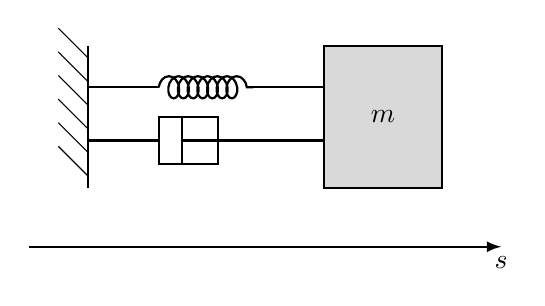
\begin{tikzpicture}[scale=1.5, >=latex]
        % Wall on the left
        \draw[thick] (0,0) -- (0,1.2);
        \foreach \i in {0.1,0.3,...,1.1} {
            \draw (0,\i) -- (-0.25,\i+0.25);
        }
        
        % Spring (upper path)
        \draw[thick] (0,0.85) -- (0.6,0.85);
        \draw[thick, decorate, decoration={coil,aspect=0.7,segment length=3.5pt, amplitude=4pt}] (0.6,0.85) -- (1.4,0.85);
        \draw[thick] (1.4,0.85) -- (2,0.85);
        
        %damper (lower path)
        \draw[thick] (0, 0.4) -- (0.6, 0.4);
        \draw[thick] (0.6,0.2) rectangle (1.1, 0.6);
        \draw[thick] (0.8, 0.4) -- (1.1, 0.4);
        \draw[thick] (0.8, 0.2) -- (0.8, 0.6);
        \draw[thick] (1.1, 0.4) -- (2, 0.4);
        % Mass box
        \draw[thick, fill=gray!30] (2,0) rectangle (3,1.2);
        \node at (2.5,0.6) {$m$};
        
        % x-axis at bottom
        \draw[thick, ->] (-0.5,-0.5) -- (3.5,-0.5);
        \node[below] at (3.5,-0.5) {$s$};
    \end{tikzpicture}
    \caption{Mass-spring-damper system}
    \label{fig:spring-mass}
\end{figure}

The MATLAB implementation of the system started off from Newton's second law:
\begin{equation}
    F = ma
\end{equation}
Knowing that the forces acting on the mass are the spring force $F_s = -ks$ and
the damping force $F_d = -cv$, the governing equation of the system can be written as:
\begin{equation}
    -k \cdot s - c \cdot v = m \cdot a
\end{equation}
This can be rearranged to express the acceleration:
\begin{equation}
    a = -\frac{k}{m} \cdot s - \frac{c}{m} \cdot v
\end{equation}

Next, by choosing specific values for the parameters $m$, $k$, and $c$, the ideal
system was simulated in MATLAB to generate measurement data for s, as in a real scenario,
it is most likely that only the position of the mass can be measured, the velocity and
acceleration would have to be estimated from the position data.\par
The chosen parameters, initial conditions and simulation settings were:
\begin{itemize}
    \item Mass $m = 1$ [kg]
    \item Spring constant $k = 4$ [N/m]
    \item Damping constant $c = 0.8$ [Ns/m]
    \item Initial position $s(1) = 1$ [m]
    \item Initial velocity $v(1) = 0$ [m/s]
    \item Simulation time $t = 0$ to $15$ [seconds] with a time step of $0.01$ [seconds]
\end{itemize}

\newpage

The plot of the idealsimulated position, velocity and acceleration data is shown
in Figure \ref{fig:spring-mass-data}.\par
\begin{figure}[H]
    \centering
    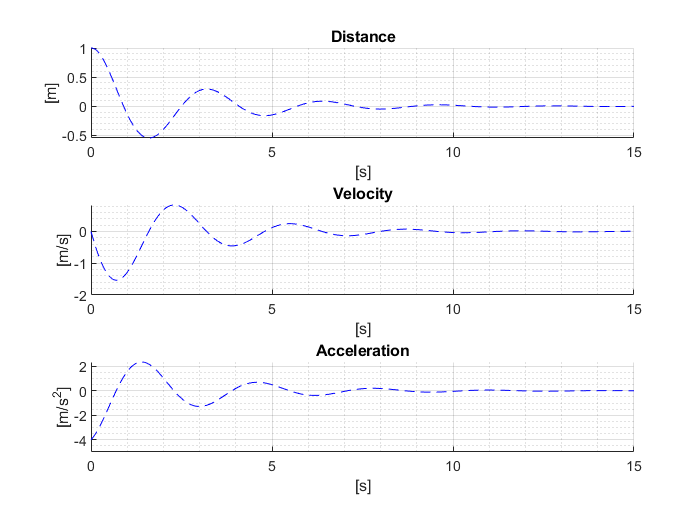
\includegraphics[width=0.6\textwidth]{spring_mass_data.png}
    \caption{Simulated ideal position, velocity, and acceleration data for the spring-mass-damper system}
    \label{fig:spring-mass-data}
\end{figure}

Next, noise was added to the position data (gaussian with a noise level of 0.00001)
to simulate measurement noise, the velocity and
acceleration were estimated from the noisy position data using the diff() function, 
which calculates the difference between consecutive elements.The same principle was applied 
to the velocity data to estimate the acceleration. The resultsare shown in
Figure \ref{fig:spring-mass-noisy-data}.\par 
\begin{figure}[H]
    \centering
    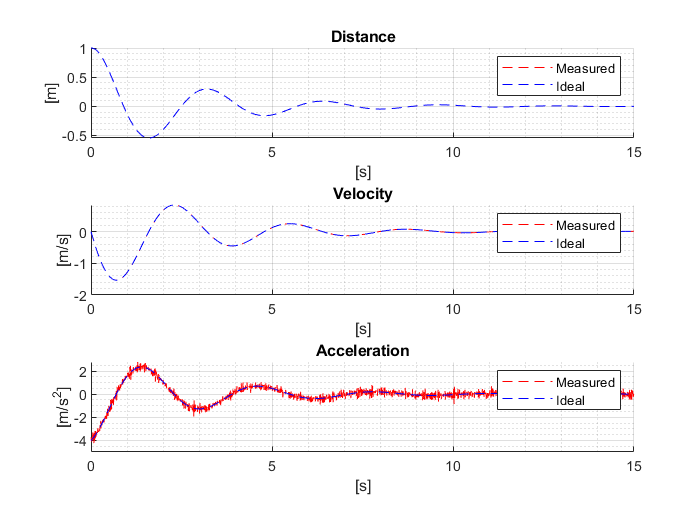
\includegraphics[width=0.6\textwidth]{spring_mass_noisy_data.png}
    \caption{Simulated noisy position, velocity, and acceleration data for the spring-mass-damper system}
    \label{fig:spring-mass-noisy-data}
\end{figure}
As it can be seen, even this little noise becomes singificant in the acceleration data,
because of the numerical differentiation.\par

Next, it was time to test SINDy on the noisy "measurement" data.
A library of candidate functions was constructed:
\begin{equation}
    \bm{\Theta}(\bm{X}) = \begin{bmatrix}
    1 & s & v & vs & v^2 & s^2 & s^2v & sv^2 & s^3 & v^3
    \end{bmatrix}
\end{equation}

The library was normalized with the RMS of each column for the $\bm{\Xi}$ coefficients to be
comparable, and the regression was applied to determine the coefficients for each 
candidate function.\par

This way, the results for $\bm{\Xi}$ are the following 
(of course, the results may differ on each run because of the noise):

\begin{equation}
    \bm{\Xi} = \begin{bmatrix}
   0.0001 \\
   -0.3377 \\
   -0.8990 \\
   -0.0046 \\
   -0.0007 \\
   -0.0025 \\
   -0.0048 \\
   -0.0054 \\
   -0.0046 \\
    0.0015 \\
    \end{bmatrix}
\end{equation}  

\newpage
\printbibliography

\end{document}

